% Options for packages loaded elsewhere
\PassOptionsToPackage{unicode}{hyperref}
\PassOptionsToPackage{hyphens}{url}
\PassOptionsToPackage{dvipsnames,svgnames,x11names}{xcolor}
%
\documentclass[
  12pt,
  a4paper,
]{scrreprt}

\usepackage{amsmath,amssymb}
\usepackage{iftex}
\ifPDFTeX
  \usepackage[T1]{fontenc}
  \usepackage[utf8]{inputenc}
  \usepackage{textcomp} % provide euro and other symbols
\else % if luatex or xetex
  \usepackage{unicode-math}
  \defaultfontfeatures{Scale=MatchLowercase}
  \defaultfontfeatures[\rmfamily]{Ligatures=TeX,Scale=1}
\fi
\usepackage{lmodern}
\ifPDFTeX\else  
    % xetex/luatex font selection
\fi
% Use upquote if available, for straight quotes in verbatim environments
\IfFileExists{upquote.sty}{\usepackage{upquote}}{}
\IfFileExists{microtype.sty}{% use microtype if available
  \usepackage[]{microtype}
  \UseMicrotypeSet[protrusion]{basicmath} % disable protrusion for tt fonts
}{}
\usepackage{xcolor}
\usepackage[left=3cm,,right=2cm,,top=3cm,,bottom=2cm]{geometry}
\setlength{\emergencystretch}{3em} % prevent overfull lines
\setcounter{secnumdepth}{5}


\providecommand{\tightlist}{%
  \setlength{\itemsep}{0pt}\setlength{\parskip}{0pt}}\usepackage{longtable,booktabs,array}
\usepackage{calc} % for calculating minipage widths
% Correct order of tables after \paragraph or \subparagraph
\usepackage{etoolbox}
\makeatletter
\patchcmd\longtable{\par}{\if@noskipsec\mbox{}\fi\par}{}{}
\makeatother
% Allow footnotes in longtable head/foot
\IfFileExists{footnotehyper.sty}{\usepackage{footnotehyper}}{\usepackage{footnote}}
\makesavenoteenv{longtable}
\usepackage{graphicx}
\makeatletter
\newsavebox\pandoc@box
\newcommand*\pandocbounded[1]{% scales image to fit in text height/width
  \sbox\pandoc@box{#1}%
  \Gscale@div\@tempa{\textheight}{\dimexpr\ht\pandoc@box+\dp\pandoc@box\relax}%
  \Gscale@div\@tempb{\linewidth}{\wd\pandoc@box}%
  \ifdim\@tempb\p@<\@tempa\p@\let\@tempa\@tempb\fi% select the smaller of both
  \ifdim\@tempa\p@<\p@\scalebox{\@tempa}{\usebox\pandoc@box}%
  \else\usebox{\pandoc@box}%
  \fi%
}
% Set default figure placement to htbp
\def\fps@figure{htbp}
\makeatother

\usepackage{dirtree}
\usepackage{amsmath}
\usepackage[explicit]{titlesec}
\usepackage{setspace}
\usepackage{caption}
\usepackage[hang,flushmargin]{footmisc}
\usepackage{etoolbox}
\usepackage[shortlabels]{enumitem}
\usepackage{booktabs}
\usepackage{ragged2e}
\usepackage{pdflscape}
\usepackage{fancyhdr}

\newcommand{\blandscape}{\begin{landscape}}
\newcommand{\elandscape}{\end{landscape}}
\renewcommand{\footnotesize}{\scriptsize}
\renewcommand{\footnoterule}{\noindent\rule{5cm}{0.4pt}\vspace{0.2cm}}
\setlength{\footnotesep}{0.5em}

\setlength{\parskip}{0.0em}
\AtBeginEnvironment{quote}{\setstretch{1.0}}

\titleformat{\section}{\normalfont\large\bfseries}{}{0pt}{\thesection\quad#1}[]
\titleformat{\subsection}{\normalfont\normalsize\bfseries}{}{0pt}{\thesubsection\quad#1}[]
\titleformat{\subsubsection}{\normalfont\normalsize\itshape}{}{0pt}{#1}[]
\titleformat{\paragraph}[runin]{\normalfont\normalsize\bfseries}{}{0pt}{#1}[]
\titleformat{\subparagraph}[runin]{\normalfont\normalsize\itshape}{}{0pt}{#1}[]

\titlespacing*{\section}{0pt}{20pt}{10pt}
\titlespacing*{\subsection}{0pt}{15pt}{10pt}
\titlespacing*{\subsubsection}{0pt}{10pt}{10pt}
\titlespacing*{\paragraph}{0pt}{10pt}{10pt}
\titlespacing*{\subparagraph}{0pt}{10pt}{10pt}
\makeatletter
\@ifpackageloaded{caption}{}{\usepackage{caption}}
\AtBeginDocument{%
\ifdefined\contentsname
  \renewcommand*\contentsname{Índice}
\else
  \newcommand\contentsname{Índice}
\fi
\ifdefined\listfigurename
  \renewcommand*\listfigurename{Lista de Figuras}
\else
  \newcommand\listfigurename{Lista de Figuras}
\fi
\ifdefined\listtablename
  \renewcommand*\listtablename{Lista de Tabelas}
\else
  \newcommand\listtablename{Lista de Tabelas}
\fi
\ifdefined\figurename
  \renewcommand*\figurename{Figura}
\else
  \newcommand\figurename{Figura}
\fi
\ifdefined\tablename
  \renewcommand*\tablename{Tabela}
\else
  \newcommand\tablename{Tabela}
\fi
}
\@ifpackageloaded{float}{}{\usepackage{float}}
\floatstyle{ruled}
\@ifundefined{c@chapter}{\newfloat{codelisting}{h}{lop}}{\newfloat{codelisting}{h}{lop}[chapter]}
\floatname{codelisting}{Listagem}
\newcommand*\listoflistings{\listof{codelisting}{Lista de Listagens}}
\makeatother
\makeatletter
\makeatother
\makeatletter
\@ifpackageloaded{caption}{}{\usepackage{caption}}
\@ifpackageloaded{subcaption}{}{\usepackage{subcaption}}
\makeatother
\makeatletter
\@ifpackageloaded{tcolorbox}{}{\usepackage[skins,breakable]{tcolorbox}}
\makeatother
\makeatletter
\@ifundefined{shadecolor}{\definecolor{shadecolor}{rgb}{.97, .97, .97}}{}
\makeatother
\makeatletter
\@ifundefined{codebgcolor}{\definecolor{codebgcolor}{HTML}{F0F2F4}}{}
\makeatother
\makeatletter
\ifdefined\Shaded\renewenvironment{Shaded}{\begin{tcolorbox}[frame hidden, boxrule=0pt, enhanced, colback={codebgcolor}, sharp corners, breakable]}{\end{tcolorbox}}\fi
\makeatother

\ifLuaTeX
\usepackage[bidi=basic]{babel}
\else
\usepackage[bidi=default]{babel}
\fi
\babelprovide[main,import]{brazilian}
% get rid of language-specific shorthands (see #6817):
\let\LanguageShortHands\languageshorthands
\def\languageshorthands#1{}
\usepackage{bookmark}

\IfFileExists{xurl.sty}{\usepackage{xurl}}{} % add URL line breaks if available
\urlstyle{same} % disable monospaced font for URLs
\hypersetup{
  pdftitle={Segundo relatório da disciplina de demografia II - Roraima},
  pdfauthor={Gabriel de Jesus Pereira},
  pdflang={pt-br},
  colorlinks=true,
  linkcolor={blue},
  filecolor={Maroon},
  citecolor={Blue},
  urlcolor={Blue},
  pdfcreator={LaTeX via pandoc}}


\title{Segundo relatório da disciplina de demografia II - Roraima}
\author{Gabriel de Jesus Pereira}
\date{abril, 2025}

\begin{document}
\cleardoublepage
\thispagestyle{empty}
{\centering
\noindent\rule{\textwidth}{0.5pt}

\vspace{2ex}

{\Large\bfseries Universidade Federal da Paraíba \par}
\vspace{1ex}
{\Large\bfseries Centro de Ciências Exatas e da Natureza \par}
\vspace{1ex}
{\Large\bfseries Departamento de Estatística \par}

\vfill

{\large\bfseries Segundo relatório da disciplina de demografia II -
Roraima \par}

\vfill

{\large Gabriel de Jesus Pereira \par}
\vfill
{\normalsize abril, 2025 \par}


\noindent\rule{\textwidth}{0.5pt}

}
\renewcommand*\contentsname{\centering Sumário \thispagestyle{empty}}
{
\hypersetup{linkcolor=}
\setcounter{tocdepth}{2}
\tableofcontents
}

\pagenumbering{arabic}
\pagestyle{fancy}

\fancyhf{}
\fancyhead[RO, LE]{\thepage}
\fancyhead[LO]{\leftmark}
\fancyhead[RE]{\thepage}

\fancypagestyle{plain}{
  \pagestyle{fancy}
  \fancyhf{}
  \fancyhead[RO, LE]{\thepage}
  \fancyhead[RE]{\thepage}
  \renewcommand{\headrulewidth}{0pt}
}

\chapter{Introdução}\label{introduuxe7uxe3o}

\section{Recursos computacionais}\label{recursos-computacionais}

\chapter{Metodologia}\label{metodologia}

\section{Técnica de sobrevivência de
Brass}\label{tuxe9cnica-de-sobrevivuxeancia-de-brass}

A técnica de sobrevivência de Brass, proposta por William Brass, é um
método indireto utilizado para estimar níveis de mortalidade infantil e
na infância em populações com dados vitais incompletos ou de baixa
qualidade. O método baseia-se em informações obtidas a partir de censos
ou pesquisas domiciliares, onde as mulheres são questionadas sobre
número de filhos nascidos vivos e número de filhos sobreviventes na data
do censo por grupos de idade das mulheres, em diferentes faixas etárias
reprodutivas.

\vspace{12pt}

Para sua aplicação, o método de Brass pressupõe algumas características.
Por exemplo, A fecundidade específica por idade tem sido aproximadamente
constante no passado recente, coeficientes de mortalidade infantil e na
infância têm sido aproximadamente constantes, não há acentuada
associação entre mortalidade infantil e idade da mãe ou entre os
coeficientes de mortalidade das mães e dos seus filhos, taxas de
subenumeração para crianças sobreviventes e não sobreviventes são
aproximadamente iguais. Por último, O ``padrão etário'' de mortalidade
para idades jovens segue aproximadamente os padrões das tábuas-modelo

\vspace{12pt}

o princípio do método é que, conhecendo o número de filhos nascidos e o
número de filhos sobreviventes, é possível calcular a proporção de
filhos falecidos para cada grupo etário de mães. Essa proporção reflete
indiretamente o nível de mortalidade infantil, já que mulheres mais
velhas, por exemplo, tiveram filhos há mais tempo, e portanto o risco
acumulado de morte é maior entre seus filhos.

\vspace{12pt}

A fórmula básica usada é:

\[
D_i = 1 - \frac{\text{FV}_i}{\text{FNV}_i}\text{, }
\] em que \(\text{FV}_i\) é o número de filhos sobreviventes na data do
censo por grupos de idade das mulheres e \(\text{FNV}_i\) é o número de
nascidos vivos por grupo etário das mulheres.

\vspace{12pt}

Utilizando-se a relação entre a proporção de filhos mortos, \(D_i\), e a
probabilidade de morrer da tábua de vida, \(q_x\), Brass estabeleceu um
conjunto de multiplicadores, \(k_i\), que podem ser calculados a partir
de interpolação linear a partir da tabela padrão a seguir:

\begin{figure}[H]

{\centering \pandocbounded{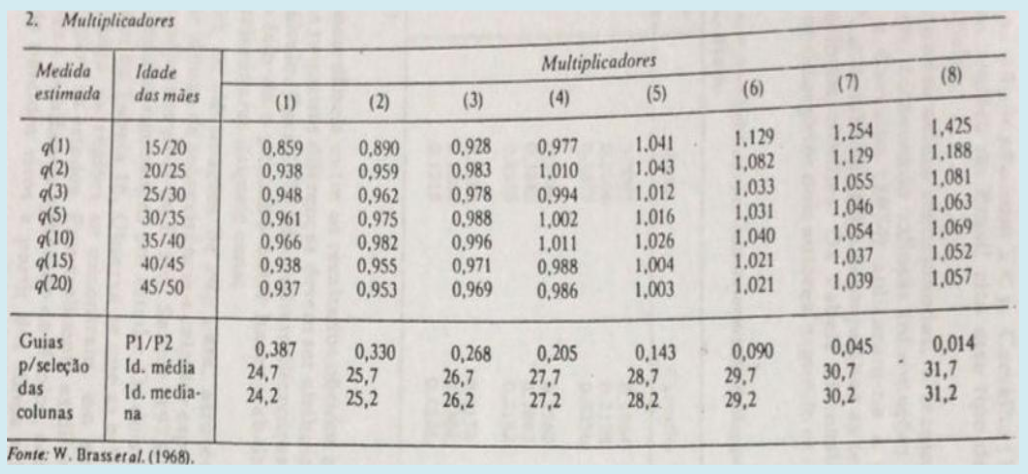
\includegraphics[keepaspectratio]{includes/sob_brass.png}}

}

\caption{Tabela para determinação de multiplicadores \(k_i\).}

\end{figure}%

Agora, com esses valores \(k_i\), pode-se converter os valores
observados \(D_i\) em estimativas de \(q_x\), ou seja, probabilidade de
morte entre o nascimento e idades exatas:

\[
q_x = k_i D_i\text{.}
\]

Tendo estimado o conjunto de probabilidades de morte \(q_x\), obtém-se,
por diferença, a probabilidade de sobrevivência entre o nascimento e
idades exatas, \(I_x\):

\[
I_x = I - q_x\text{.}
\]

\section{Técnica de Brass para estimar a
fecundidade}\label{tuxe9cnica-de-brass-para-estimar-a-fecundidade}

~~~O objetivo da técnica de Brass estimar a fecundidade é estimar a
fecundidade em países cujos dados de registro civil não permitem um
cálculo razoável do seu nível.

\vspace{12pt}

Um de seus pressupostos parar aplicação do método é que a fecundidade
tenha sido aproximadamente constante no passado recente. Além desse
pressuposto, é necessário também que os coeficientes específicos de
fecundidade por idade da mulher, tais como os obtidos através de
perguntas diretas, são corretos quanto ao padrão etário da fecundidade e
o nível de fecundidade é corretamente medido através do número de filhos
tidos (nascidos vivos) informados pelas mulheres mais jovens (usualmente
do grupo etário 20-25) -- ou seja, através da parturição média dessas
mulheres.

\vspace{12pt}

Para utilizar a técnica de Brass, será necessário calcular os nascidos
vivos no ano anterior ao censo por mulher, que é denotado por \(f_i\),
total de nascidos vivos por mulher \(P_i\). A partir de \(f_i\),
calcula-se a fucundidade acumulada no começo do intervalo
\(F^{'}_i = 5 \sum_{j=0}^{i-1} f_{j}\). Uma das outras componentes que
compõe o método são os fatores de multiplicação \(W_i\), que são valores
tabelados e que podem ser calculados por interporlação linear a partir
do intervalo que \(f_{1}/f_{2}\) estão definidos na tabela a seguir:

\begin{figure}[H]

{\centering \pandocbounded{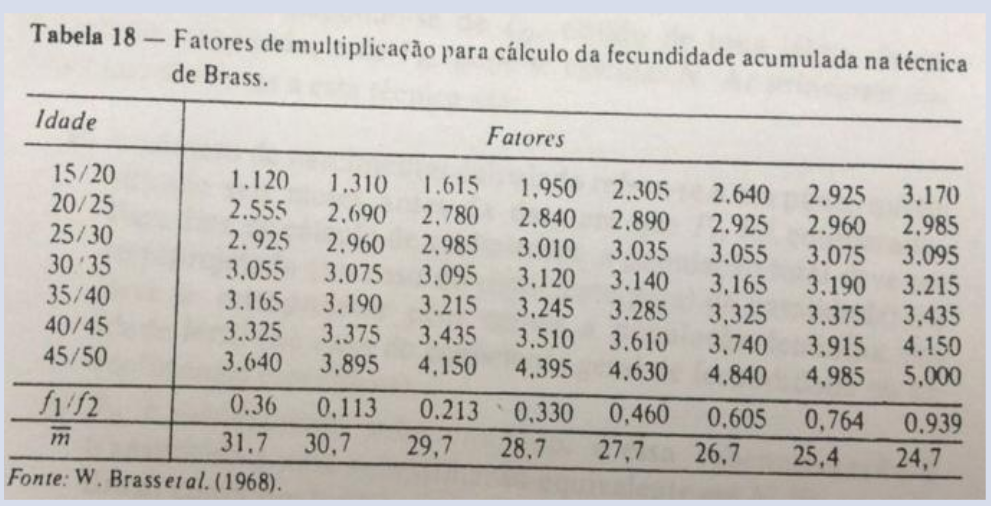
\includegraphics[keepaspectratio]{includes/fatores_mult.png}}

}

\caption{Valores tabelados para cálculo de fatores de multiplicação
\(W_i\).}

\end{figure}%

Após encontrar os fatores de multiplicação \(W_i\), basta cálcular a
fecundidade acumulada média com \(F_i =  F_i + W_if_i\). Por fim,
encontram-se os coeficientes específicos corrigidos
\(f^{'}=f_iP_{2}/F_{2}\).

\section{Modelando taxa de fecundidade
marital}\label{modelando-taxa-de-fecundidade-marital}

~~~O modelo de fecundidade marital de Coale-Trussell é uma das
abordagens clássicas para estudar o comportamento reprodutivo de
mulheres casadas, oferecendo uma maneira prática de estimar e
interpretar padrões de fecundidade observados com base em uma
curva-padrão e parâmetros de ajuste. Sua aplicação é especialmente útil
em estudos demográficos comparativos entre diferentes regiões ou ao
longo do tempo.

\vspace{12pt}

O modelo parte da ideia de que a fecundidade marital observada pode ser
representada como uma modificação de um padrão considerado ``natural''
ou ``biológico'' de fecundidade. A fórmula principal é:

\[
f\left(a\right) = G\left(a\right) r\left(a\right)\text{, }
\] em que \(a\) é a idade, \(f\left(a\right)\) é a taxa específica de
fecundidade, \(G\left(a\right)\) é o risco do primeiro casamento,
\(r\left(a\right)\) é a taxa específica de fecundidade marital, a qual é
expressa da seguinte forma:

\[
r\left(a\right) = M n\left(a\right) e^{m v\left(a\right)} \text{, }
\] em que \(M\) é o nível de fecundidade e \(m\) é o padrão de
fecundidade. \(n\left(a\right)\) é a fecundidade marital natural e
\(v\left(a\right)\) é a fecundidade fixa.

\vspace{12pt}

Por fim, a partir da expressão de \(r\left(a\right)\) pode ser definida
uma regressão linear da seguinte forma:

\[
\ln\left(r\left(a\right) / n\left(a\right)\right) = \ln\left(M\right) + mv\left(a\right)
\]

\vspace{12pt}

Além disso, vale ressaltar que a fecundidade marital e natural e a
fecundidade fixa são derivadas por experiência de alguns países,
principalmente europeus. A imagem a seguir mostra os valores que foram
considerados para esse trabalho:

\begin{figure}[H]

{\centering \pandocbounded{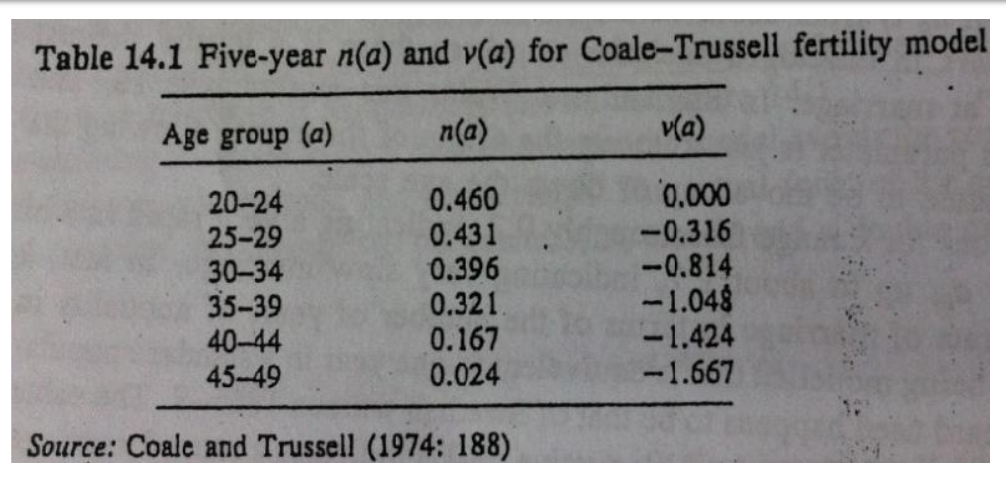
\includegraphics[keepaspectratio]{includes/tabela_coell.png}}

}

\caption{Valores tabelados de \(n\left(a\right)\) e \(v\left(a\right)\)
para aplicação do método de Coale-Trussel.}

\end{figure}%

\section{Modelo relacional de
Gompertz}\label{modelo-relacional-de-gompertz}

~~~O modelo relacional de Gompertz é uma metodologia demográfica
amplamente utilizada para descrever e ajustar padrões de fecundidade,
especialmente quando os dados observados apresentam problemas de
cobertura ou qualidade. Sua principal utilidade está em permitir
comparações entre diferentes populações ou períodos por meio de uma
curva-padrão acumulada de fecundidade.

\vspace{12pt}

A lógica do modelo baseia-se na função de Gompertz, originalmente
utilizada para modelar taxas de mortalidade, mas que também pode ser
aplicada ao padrão acumulado da fecundidade, \(F\left(a\right)\), isto
é, a proporção da fecundidade total que já ocorreu até determinada idade
\(a\). O modelo assume a seguinte forma funcional:

\[
\text{Gompit}\left(F\left(a\right)\right) = \ln\left[-\ln\left(1-F\left(a\right)\right)\right] = \alpha + \beta\text{Gompit}\left(F_{s}\left(a\right)\right)
\] em que \(F\left(a\right)\) é a distribuição acumulada de fecundidade
da população observada, \(F_{s}\left(a\right)\) é a distribuição
acumulada de fecundidade da população padrão, \(-0,5< \alpha < 0,5\) e
\(0,65 < \beta < 1,5\) são o nível da fecundidade e padrão da
fecundidade, respectivamente.

\vspace{12pt}

Para aplicar o modelo, é necessário calcular a distribuição proporcional
das taxas específicas de fecundidade \(p\left(a\right)\), obter a
distribuição acumulada \(F\left(a\right)\), aplicar a transformação
Gompit \(\ln\left[-\ln\left(1 - F\left(a\right)\right)\right]\), ajustar
uma regressão linear entre os gompits da população observada e os da
curva padrão e, por fim, estimar os parâmetros \(\alpha\) e \(\beta\),
que permitem reconstruir a curva ajustada ou fazer comparações com
outras populações.

\chapter{Resultados}\label{resultados}

\section{Técnica de sobrevivência de
Brass}\label{tuxe9cnica-de-sobrevivuxeancia-de-brass-1}

\section{Técnica de Brass para a
fecundidade}\label{tuxe9cnica-de-brass-para-a-fecundidade}

\(0.096731 / 0.134156 = 0.721033721935657\)

\((0.764 - 0.721033721935657) / (0.764 - 0.605) = 0.2702281639266858\)

\section{Modelando taxa de fecundidade
marital}\label{modelando-taxa-de-fecundidade-marital-1}

\section{Modelo relacional de
Gompertz}\label{modelo-relacional-de-gompertz-1}

\chapter{Exercícios do Mortpak}\label{exercuxedcios-do-mortpak}

\begin{figure}

\begin{minipage}{\linewidth}

\begin{figure}[H]

{\centering \pandocbounded{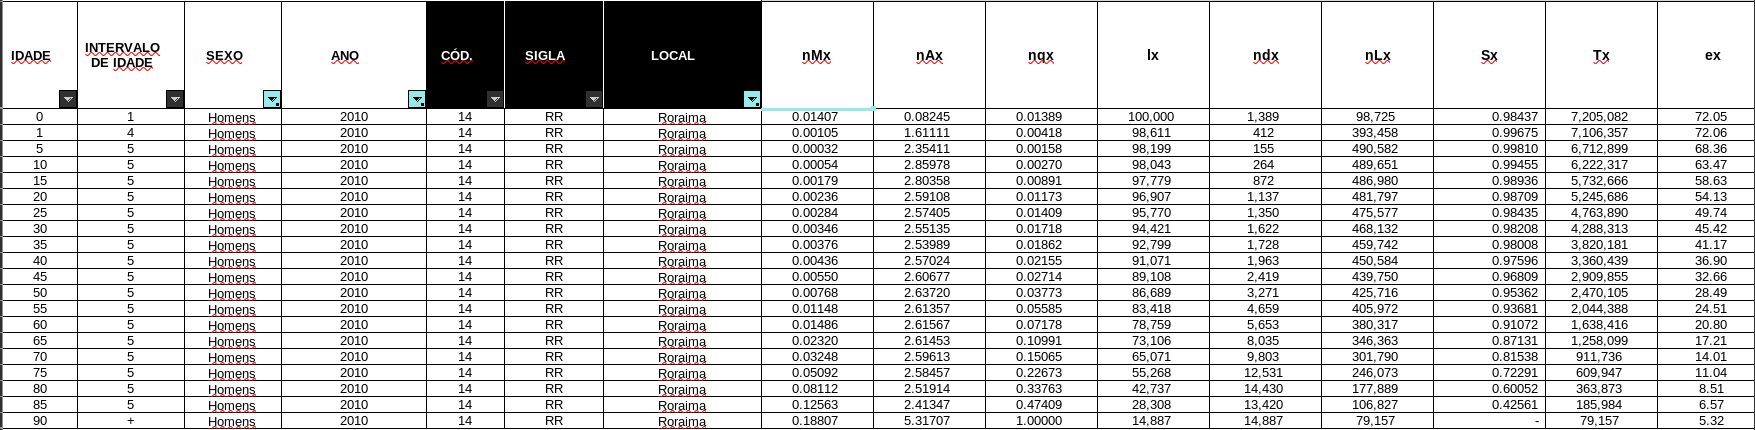
\includegraphics[keepaspectratio]{includes/tabua_vida_homens.png}}

}

\subcaption{Tábua de vida para o sexo masculino.}

\end{figure}%

\end{minipage}%
\newline
\begin{minipage}{\linewidth}

\begin{figure}[H]

{\centering \pandocbounded{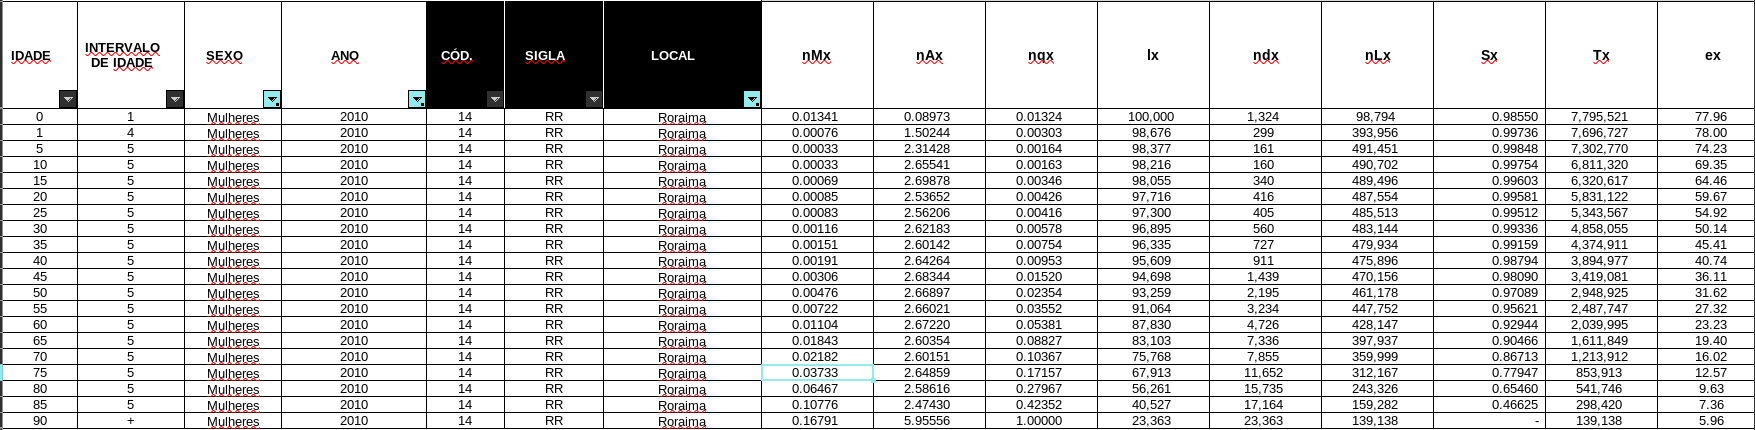
\includegraphics[keepaspectratio]{includes/tabua_vida_mulheres.png}}

}

\subcaption{Tábua de vida para o sexo feminino.}

\end{figure}%

\end{minipage}%

\end{figure}%

\section{Questão 1)}\label{questuxe3o-1}

Ver no Mortpak qual é o melhor modelo ao comparar os Modelos das Nações
Unidas aos de Coale-Demeny (Função COMPAR);

\begin{figure}

\begin{minipage}{0.50\linewidth}

\begin{figure}[H]

{\centering \pandocbounded{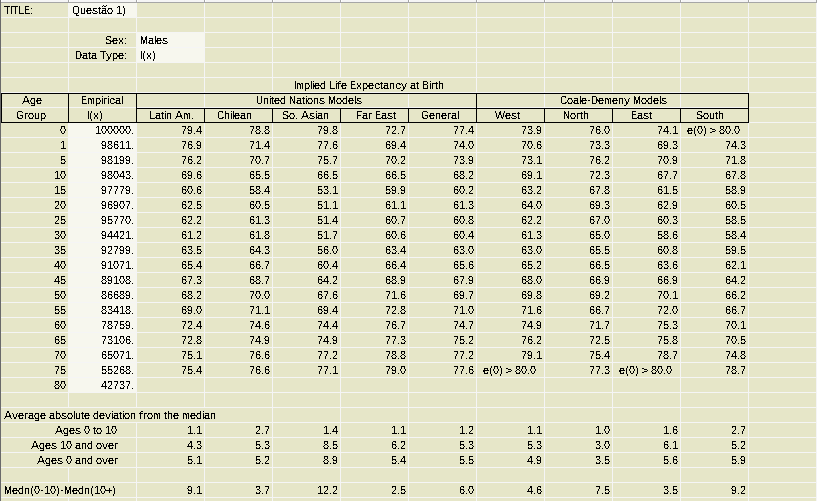
\includegraphics[keepaspectratio]{includes/expec_vida_homens.png}}

}

\subcaption{Função COMPAR para o sexo masculino.}

\end{figure}%

\end{minipage}%
%
\begin{minipage}{0.50\linewidth}

\begin{figure}[H]

{\centering \pandocbounded{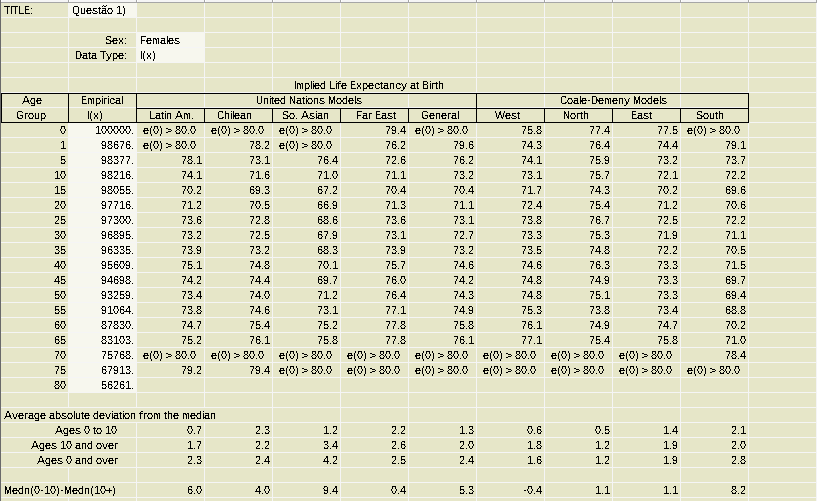
\includegraphics[keepaspectratio]{includes/expec_vida_mulheres.png}}

}

\subcaption{Função COMPAR para o sexo feminino.}

\end{figure}%

\end{minipage}%

\end{figure}%

\section{Questão 2)}\label{questuxe3o-2}

Considerar apenas os Modelos das Nações Unidas e ver qual é o melhor
(Função COMPAR);

\section{Questão 3)}\label{questuxe3o-3}

Observar os valores da \(E\left(x\right)\) e escolher a TV Modelo das
Nações Unidas mais adequada (depende do passo 2\ldots);

\section{Questão 4)}\label{questuxe3o-4}

Usar o sistema logito de tábuas de vida de dois parâmetros de Brass e
considerar os seguintes padrões: Modelo Geral de Brass; MAB e o
resultado do passo 3.




\end{document}
